\chapter{Simulation}\label{ch13}
\section{Introduction}

One of the important benefits of using a simulator like \Le is that a circuit designer can simulate digital systems to determine logic flaws or weaknesses that must be addressed before a physical \gls{ic} is manufactured. This chapter introduces the concept of simulation and includes several examples of simulated systems. \textit{(Note: this chapter is still under development and only contains one simulated system.)}

%***************************************************************************
% Section: Elevator
%***************************************************************************
\section{Elevator}
\label{SIM:sec:elevator}

As a simple example of a \gls{ic}, imagine an elevator control circuit. For simplicity, this elevator is in a five story building and buttons like ``door open'' will be ignored. There are two ways the elevator can be called to a given floor: someone could push the floor button in the elevator car to ride to that floor or someone could push the call button beside the elevator door on a floor.

 Figure \ref{SIM:fig:elevator} is the Moore \gls{fsm} for this circuit:

\begin{figure}[H]
  \caption{Elevator}
  \label{SIM:fig:elevator}
  \myfloatalign
  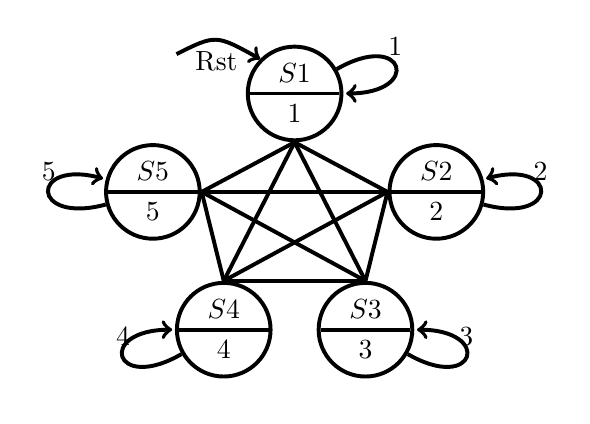
\begin{tikzpicture} [scale=1.00]
  \usepgflibrary{shapes.multipart} % for the multipart nodes
  % make all path lines (the node shapes) a little thicker
  \tikzstyle{every path}=[line width=0.50mm]  
  
  % Draw the lines
  \node [circle split,draw] (S1) at (4.00, 5.00) {$ S1 $ \nodepart{lower} $ 1 $};
  \node [circle split,draw] (S2) at (5.80, 3.75) {$ S2 $ \nodepart{lower} $ 2 $};
  \node [circle split,draw] (S3) at (4.90, 2.00) {$ S3 $ \nodepart{lower} $ 3 $};
  \node [circle split,draw] (S4) at (3.10, 2.00) {$ S4 $ \nodepart{lower} $ 4 $};
  \node [circle split,draw] (S5) at (2.20, 3.75) {$ S5 $ \nodepart{lower} $ 5 $};
  
  % edge connectors
  \draw (S1.south) -- (S2.west);
  \draw (S2.west)  -- (S3.north);
  \draw (S3.north) -- (S4.north);
  \draw (S4.north) -- (S5.east);
  \draw (S5.east)  -- (S1.south);
  % cross connectors
  \draw (S1.south) -- (S3.north);
  \draw (S1.south) -- (S4.north);
  \draw (S2.west)  -- (S5.east);
  \draw (S2.west)  -- (S4.north);
  \draw (S3.north) -- (S5.east);

  % Loops
  \draw (S1) edge [in=0,out=30,loop] node[above] {1} ();
  \draw (S2) edge [in=15,out=345,loop] node[above] {2} ();
  \draw (S3) edge [in=0,out=330,loop] node[above] {3} ();
  \draw (S4) edge [in=180,out=210,loop] node[above] {4} ();
  \draw (S5) edge [in=165,out=195,loop] node[above] {5} ();
  
  % Reset input
  \draw[->] (2.50,5.50) .. controls (3.00,5.75) .. node[below] {Rst}  (S1.north west);
    

  \end{tikzpicture}
\end{figure}

In Figure \ref{SIM:fig:elevator} the various floors are represented by the five states (S1-S5). While the elevator is at a floor then the output from the circuit is the floor number. The elevator is quiescent while in any one state and if a user pushes the button for that same floor then nothing will happen, which is illustrated by the loops starting and coming back to the same state. The star pattern in the middle of the \gls{fsm} illustrates that the elevator can move directly from one state to any other state. Finally, a Reset signal will automatically move the elevator to state S1.


